\documentclass{scrartcl}
\usepackage[utf8]{inputenc}
\usepackage{circuitikz}
\usepackage{pxfonts}
\usepackage{graphicx}
\usepackage{float}
\usepackage[ngerman]{babel}

\begin{document}

\begin{titlepage}

	\pagestyle{empty}
	\title{
\includegraphics[width=1\textwidth]{HTW.pdf}}
	\subtitle{Belegarbeit Computergrafik I \\Wintersemester 2021/22}
	\author{Felix Müller}
	\maketitle

\end{titlepage}

\tableofcontents
\listoffigures

\section{Aufgabenstellung}

Schreiben Sie ein Programm in C/C++, das unter Verwendung von OpenGL, Vertex- und
Fragment-Shadern folgende Aufgaben realisiert.

\subsection{Geometrische Objekte}
Erzeugen Sie eine interaktive zeitlich animierte Szene mit mehreren
unterschiedlichen farblichen und texturierten dreidimensionalen geometrischen Objekten.

\subsection{Beleuchtung}
Beleuchten Sie die Szene mit verschiedenartigen Lichtquellen so, dass auf den
Objekten unterschiedliche Beleuchtungseffekte sichtbar werden.

\subsection{Ansicht}
Stellen Sie die Szene gleichzeitig in verschiedenen Ansichten und Projektionen in
mehreren Viewports des Anzeigefensters dar.

\subsection{Programm}
Stellen Sie das komplette Programm in Quelltextform als Visual-Studio-C/C++-
Projekt und in ausführbarer Form als exe-File derart bereit, dass die Lauffähigkeit unter MS
Windows gewährleistet ist.

\subsection{Dokumentation}
Fertigen Sie eine Systemdokumentation in Form eines pdf-Dokumentes von
etwa 10 Seiten an, die Deckblatt, Gliederung, Aufgabenbeschreibung, Lösungsansatz,
Lösungsumsetzung, Installations- und Bedienungsanleitung, einige Bildschirm-Snapshots,
Probleme, Ergebnisse, Literatur- und Quellenverzeichnis enthält.

\subsection{Abgabe}
Übergeben Sie die Ergebnisse der Aufgaben 4 und 5 zusammengefasst in einem
Verzeichnis \textsc{Name\_Vorname\_Bibliotheksnummer} an den Lehrenden. Bei Bedarf kann sich
eine Abnahme der Belegarbeit mit Demonstration der Lauffähigkeit erforderlich machen.


\section{Lösung}

\subsection{Konstruktion der Szene}

Die Szene soll einen Baum, auf einem Waldboden zeigen. Die Spitze des Baums soll ''im Wind schwanken''.
Die Objekte der Szene sollen so beleuchtet sein, dass der Eindruck einer künstlichen Sonne entsteht. 
Zusätzlich soll ein weiteres Richtungslicht zum Einsatz kommen. 
Die Beleuchtungsstärke und die Amplitude der Bewegung der Baumspitze sollen durch Eingaben verändert werden können.
Im Programmfenster sollen drei Viewports gezeigt werden - ein statischer, ein animierter und ein interaktiver.

\subsection{Zerlegung in Objekte}

Der Baum kann in einen Kegel (Baumkrone) und einen Kegelstumpf (Baumstamm) zerlegt werden.
Der Baumstamm soll sich nach oben verjüngen.
Der Kegel kann durch Dreiecke dargestellt werden.
Der Kegelstumpf wird durch Facetten approximiert, die in je zwei Dreiecke zerlegt werden können.
Der Waldboden kann zunächst in vier gleich große Quadrate und diese in je zwei deckungsgleiche Dreiecke gegliedert werden.
Durch Anpassung der \textsc{z}-Koordinaten der Ecken kann ein Geländegefälle modelliert werden.

\subsection{Klassen}

\subsubsection{Geometrische Objekte}
Zur Berechnung der Koordinaten von Kegeln und Kegelstümpfen wurden die Klassen \textsc{Cone} und \textsc{TruncatedCone} implementiert. 
Die Berechnungsalgorithmen zur Erzeugung der Objektkoordinaten lassen sich parametrisieren, sodass die Lage der Spitze im Raum, die Höhe, der Durchmesser der Grundfläche / der Deckflächen und die Anzahl der Facetten für die Mantelfläche anpassbar sind.
Die Erzeugung der Koordinaten für den Waldboden ist durch die Klasse \textsc{Terrain} möglich.

\subsubsection{Shader und Texturen}
Um Fragment- und Vertexshader laden, kompilieren und zu einem Shaderprogramm zusammenfassen zu können gibt es die Klassen
\textsc{MyShader} und \textsc{MyShaderLoader}.
Entsprechend dient die Klasse \textsc{MyTextureLoader} dem Laden von Texturen.

\subsection{Berechnungen}

Für jeden Frame werden die Position und die Intensität des Lichts neu berechnet.
Für die \textsc{Y}-Koordinate des Sonnenlichts gilt:
$$y = f_1(\phi) = \cos(\phi)\textrm{.}$$
Für die \textsc{Z}-Koordinate gilt: 
$$z = f_2(\phi) = \cos(\phi)\textrm{.}$$

Die Lichtintensität wird anhand der Nutzereingabe bestimmt und über ein \textsc{uniform} als \textsc{float}-Wert an die Shader gereicht.
$\phi$ wird mit jedem Frame erhöht und auf $0$ gesetzt, sobald es $2\cdot\pi$ erreicht.
\\ 
Zudem wird das Schwanken der Baumspitze bestimmt. Die diesbezügliche Eingabe des Nutzers bestimmt das maximale Schwanken $L$.
Der tatsächliche Wert wird als Ausprägung einer gleichverteilten Zufallsvariable aus dem Intervall 
$0 \textrm{ bis } L$
bestimmt, damit die Bewegung möglichst natürlich wirkt.
\\
Abschließend wird die automatische Rotation der Szene im zweiten Viewport berechnet.


\section{Programmstruktur}

\begin{itemize}
	\item \textbf{void reshape(int w, int h) :} \\
	Aktualisiert die Variablen width und height für die Fenstergröße, wenn diese geändert wird.

	\item \textbf{void special(int specKey, int mouseX, int mouseY) :} \\
	Wird aufgerufen, wenn eine Pfeiltaste betätigt wird. Wurde eine Pfeiltaste betätigt, so verändert die Funktion Variablen, die die Blickposition bestimmen.
	
	\item \textbf{void keyboard( unsigned char theKey, int mouseX, int mouseY) :} \\
	Wird beim Betätigen einer Taste der Tastatur aufgerufen und verändert die Szenenparameter.

	\item \textbf{void timer(int value) :} \\
	Diese Funktion wird beim Auslösen des Timerereignis aufgerufen und ruft ihrerseits \textbf{display} auf.
	Außerdem werden in bestimmten zeitlichen Abständen die zeitlich veränderlichen und durch Nutzereingaben beeinflussbaren Parameter auf der Kommandozeile ausgegeben. 
	
	\begin{figure}[h]
 		\centering
 		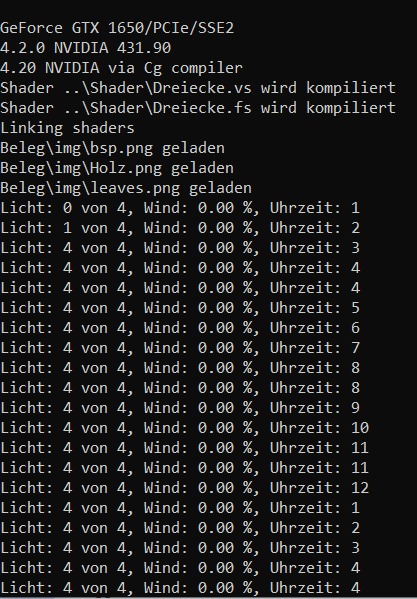
\includegraphics[width=7cm]{5.png}
 		\caption{Ausschnitt der Konsolenausgaben}
	\end{figure}

	\item \textbf{void display() :} \\
	Die Matrizen View und Projection werden entsprechend der Berechnungvorschriften für die Animation neu berechnet.
	Drei Viewports werden erzeugt und gerendert.
	
	\item \textbf{void renderScene() :} \\
	Diese Funktion dient dem neuberechnen der Objekt- und Texturkoordinaten durch die eizelnen Klassen der verschiedenen geometrischen Objekte.
	
	\item \textbf{void calcSceneParams() :} \\
	dient zum Berechnen der zeitlich veränderlichen Parameter der Szene, wie der Position des Lichts.
	
	\item \textbf{void init() :} \\
	Diese Funktion dient der Initialisierung der VAOs, VBOs und Puffern und dem Laden von Shadern und Texturen. Zudem wird die Tiefenprüfung aktiviert und die Position von Shader-Variablen bestimmt.
	
	\item \textbf{int main(int argc, char** argv) :} \\
	In dieser Funktion wird das Fenster initialisiert, die Fenstergröße festgelegt, die Callbackfunktionen für Tastatureingaben angegeben und die Renderschleife angestoßen.
		
	\item \textbf{shader.vs :} \\
	Berechnet \textsc{gl\_Position} und übergibt dem Fragment-Shader den Normalenvektor und Textur- und Vertexkoordinaten.

	\item \textbf{shader.fs :} \\
	Hier werden die Lichtwerte aus allen Lichtquellen berechnet und daraus resultierend die Farbwerte für alle Fragmente individuell festgelegt. Der Richtungsvektor der Lichtquellen wird aus Lichtposition und der Fragmentposition berechnet.

\end{itemize}

\section{Installation}

Die Projektmappe kann mit \emph{Visual Studio} geöffnet und mit folgenden Einstellungen kompiliert werden.
Wichtig sind dabei folgende zusätzliche Eingaben im Linker: \\
\emph{kernel32.lib, user32.lib, gdi32.lib, winspool.lib, comdlg32.lib, advapi32.lib, shell32.lib, ole32.lib, oleaut32.lib, uuid.lib, odbc32.lib, odbccp32.lib}\\
und folgende Include-Pfade:\\
\emph{
OpenGL//FreeImage3180Win32Win64//Dist//x32\\
OpenGL//freeglut-3.0.0//include//GL\\
OpenGL//glew-2.1.0//include//GL\\
OpenGL//glm-0.9.9.6//glm}.\\
Durch den Compile-Aufruf wird eine ausführbare Datei erzeugt, die auch ohne die Umgebung von Visual Studio ausführbar ist.

\section{Interaktivität}

Folgende Nutzereingaben beeinflussen Variablen der Szene:

\begin{itemize}
	\item die Pfeiltasten zum Bewegen des View-Points im oberen linken Viewport.
	\item \textbf{A} zum Herauszoomen und \textbf{Y} zum Hereinzoomen im oberen linken Viewport.
	\item \textbf{L} zum Steuern der Lichtintensität der ''künstlichen Sonne'' in vier Stufen.
	\item \textbf{H} zum Verstärken und \textbf{U} zum Abschwächen der Bewegung der Baumspitze.
\end{itemize}

Das Programm kann durch das Schließen des Fensters beendet werden.

\section{Screenshots}

\begin{figure}[H]
 \centering
 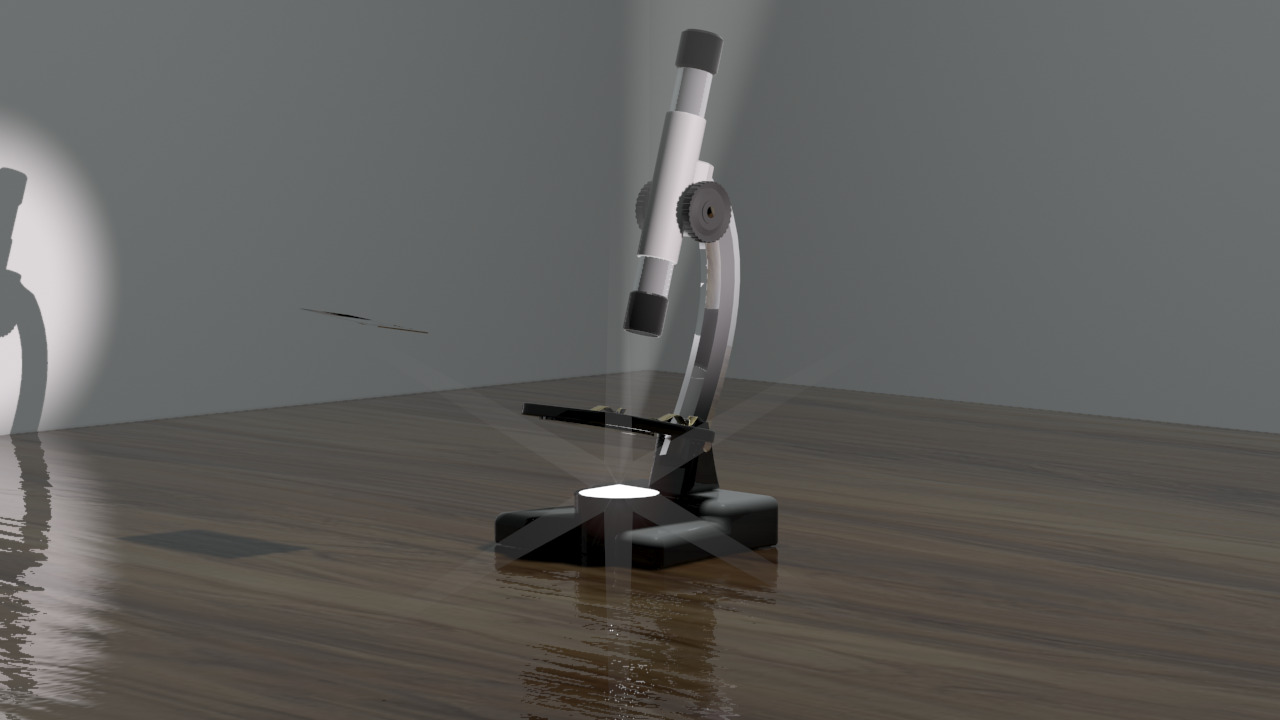
\includegraphics[width=10cm]{1.png}
 \\
 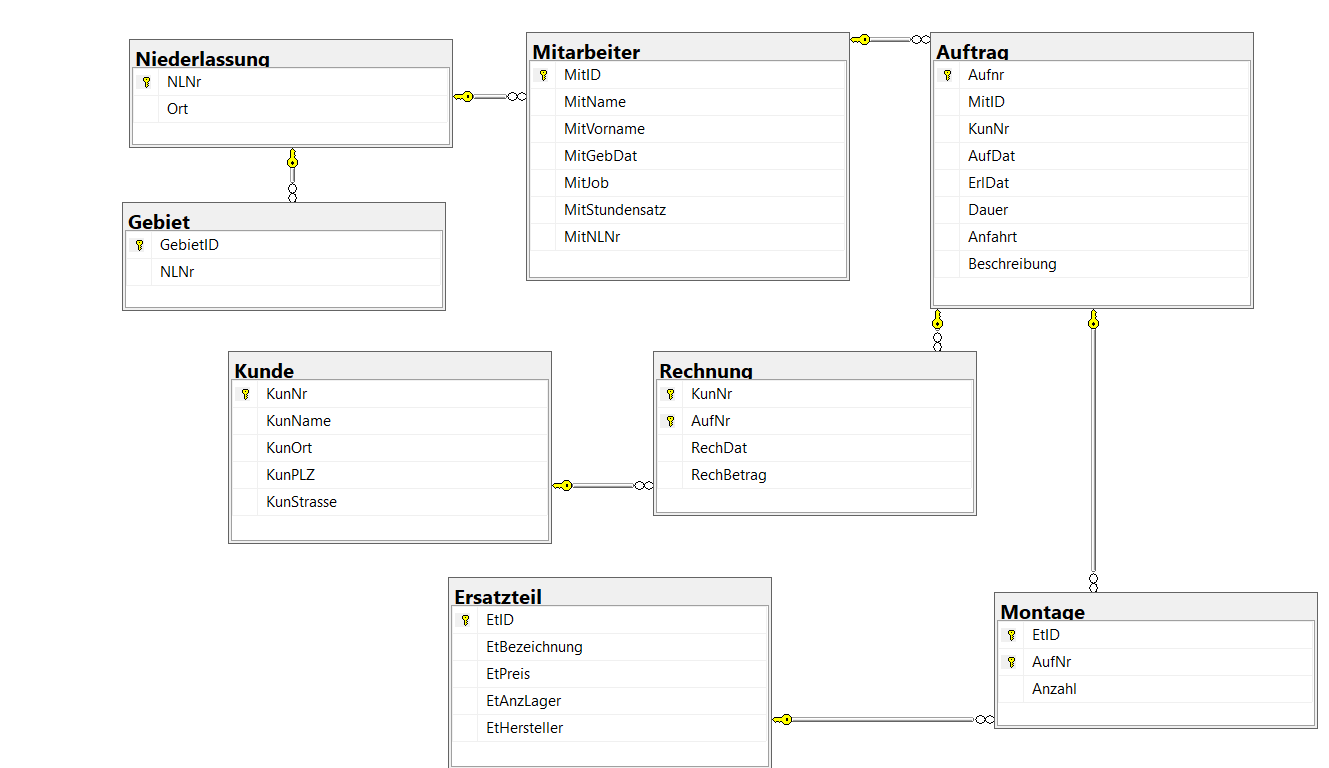
\includegraphics[width=10cm]{2.png}
 \caption{Screenshots}
\end{figure}

\section{Probleme und (Teil)-Lösungen}

\subsection{nahtlose Texturierung}

die Mantelfläche des Kegels und des Kegelstumpfs weißen Nahtstellen auf. Diese ließen sich durch spezielle nahtlose Texturen vermeiden, deren Erstellung aber aufwendig ist.

\begin{figure}[h]
 \centering
 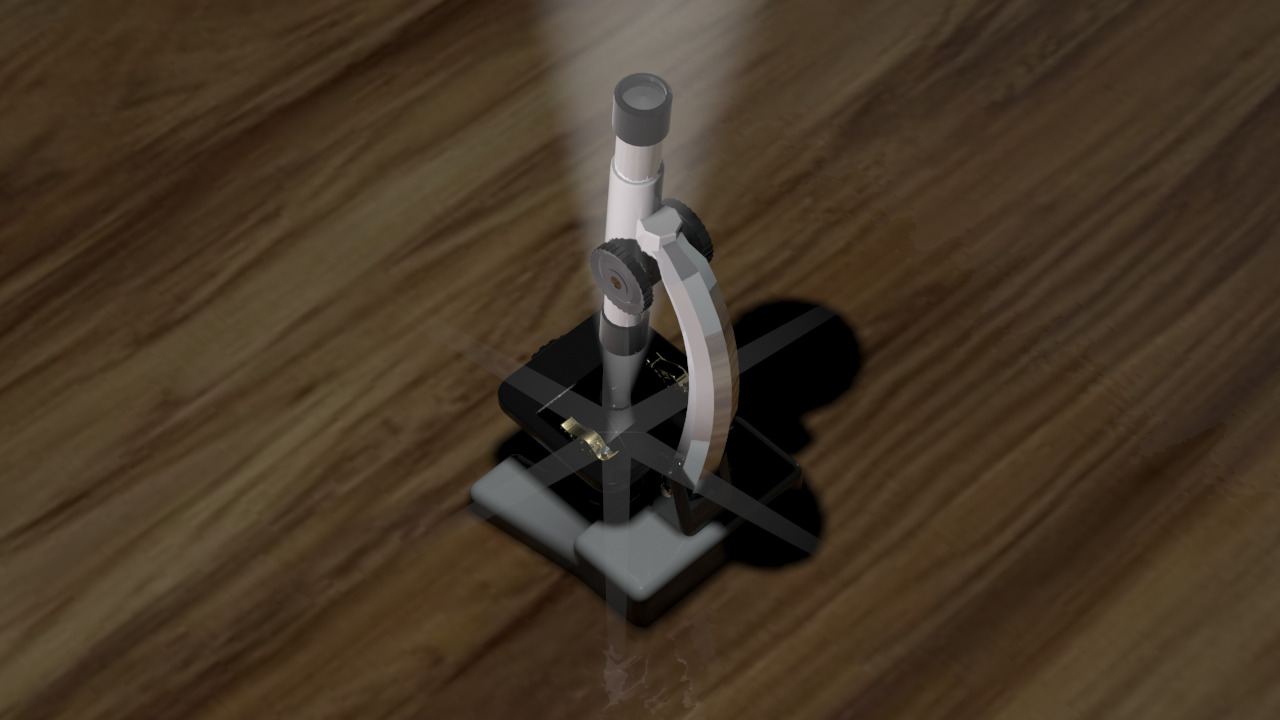
\includegraphics[width=5cm]{4.png}
 \caption{Naht in der Textur der Baumkrone}
\end{figure}



\subsection{Schatten}

Schatten wurden nicht modelliert. Damit einher geht ein Verlust an Detailtreue.

\subsection{Kollisionen}

Durch eine Begrenzung der Interaktionsmöglichkeiten über die Pfeiltasten ist das Verschieben des Blickpunktes in das Innere von Objekten nicht möglich.

\section{Literatur und Quellen}

\begin{itemize}
	\item Vorlesungsskript und Praktikumsaufgaben
	\item de Vries, Joey: Learn OpenGL - graphics programming: Learn modern OpenGL graphics programming in a step-by-step fashion, Kendall \& Welling, 2020.
	\item Kessenich,  John et al.: OpenGL Programming Guide, Addison Wesley, 2013, 8. Auflage.
\end{itemize}

\end{document}
